\section{Scientific Program}

\subsection{Background}

\subsubsection{History of Star Formation}

The detailed story of the formation of galaxies within a cosmological
framework is a major unsolved problem in contemporary cosmology
\citep[see, e.g., the recent review by][]{benson10}.  Between the end
of reionization and about 8 Gyr after the Bang, the cosmic star
formation rate density rises steadily, reaching a peak at $z\sim2.5$;
see Figure \ref{fig:ScienceCase}.  The nature of the star-forming
systems changes dramatically over this period, with the most luminous
galaxies at the peak becoming heavily dust enshrouded.  Indeed, the
discovery of the cosmic far-infrared background (CFIRB) by NASA's
\cobe\ satellite \citep{puget96,fixsen98} and the detection of a
significant population of high redshift, dust-obscured galaxies
selected at submillimeter (submm) wavelengths \citep{smail97,hughes98}
revealed that as much as half of the star formation activity in the
early Universe occurs in galaxies that are undetected at optical
wavelengths \citep{chapman05,aretxaga07}.

\begin{figure}[h]
  \begin{tabular}{ll}
    \begin{minipage}{3.25in}
      \begin{center}
	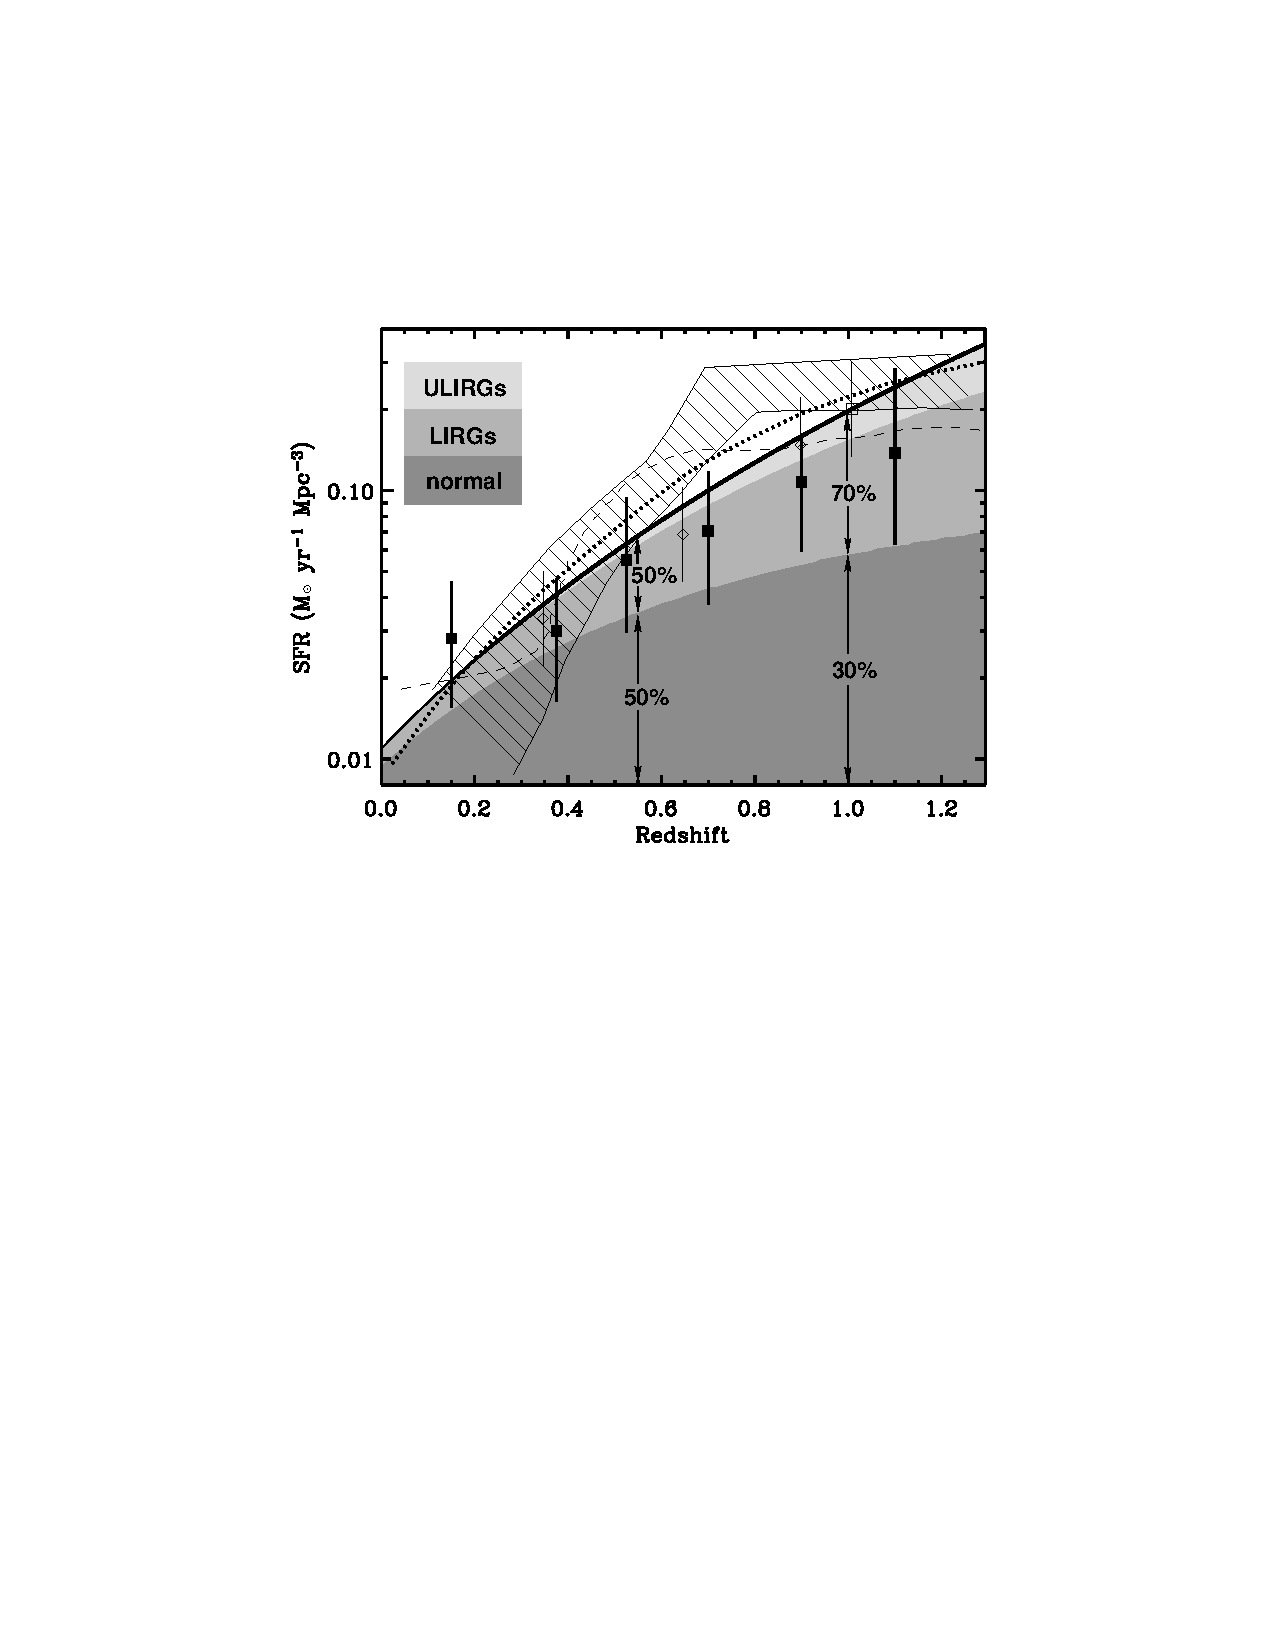
\includegraphics[width=3.25in]{lefloch04_sf_history.pdf}
%{madau_plot_somerville08.pdf}
      \end{center}     
    \end{minipage} &
    \begin{minipage}{3.25in}
      \begin{center}
	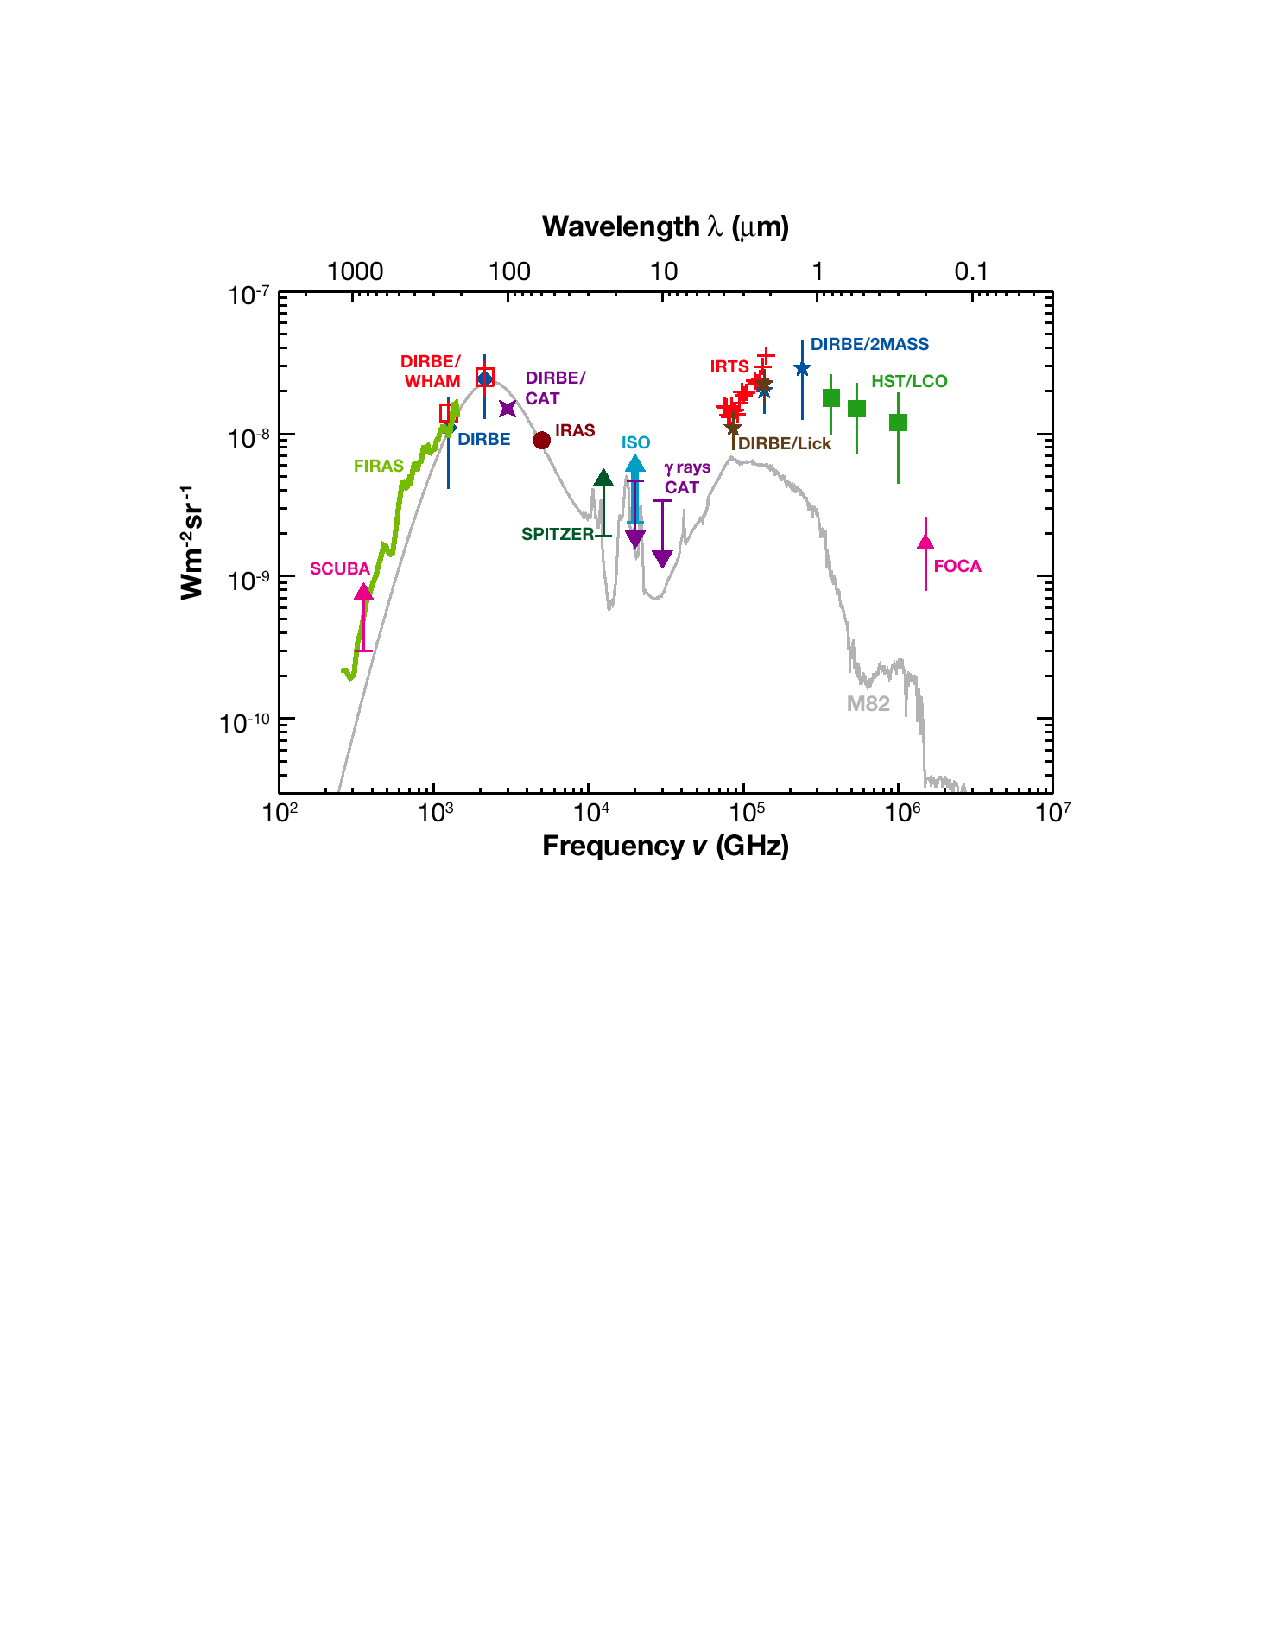
\includegraphics[width=3.25in]{lagache05_firb.pdf}
      \end{center}
    \end{minipage}
  \end{tabular}
	\captionbaseline\caption {\small {\it Left:} The evolution cosmic star
	formation rate density, broken down by the contributing
	population, from \citet{lefloch04}. {\it Right:} The fraction
	of extra-galactic background light due to far-infrared sources
	\citep{lagache05}.  Note that roughly equal amounts come from
	the optical/near-IR and far-IR.  Of the far-IR, about half the
	intensity lies at $z<1$.}
	\label{fig:ScienceCase}
\end{figure}

These (sub)millimeter-selected galaxies (hereafter SMGs) which
comprise the CFIRB are a cosmologically significant population
undergoing intense star formation (with star formation rates of up to
$\sim10^3$~M$_{\odot}$~yr$^{-1}$) when the Universe was \mbox{15 -
45\%} of its present age, between 7.5 and 11.5 billion years
ago. Optical and ultraviolet (UV) radiation from both star formation
and AGN activity heat the dust in these galaxies, and this energy is
thermally re-radiated at far-infrared (far-IR) to mm wavelengths, with
the peak of dust emission occurring at $\sim60-200\,\mu$m in the
rest-frame \citep{soifer91}.  The large amount of dust present in them
often precludes detailed study at optical wavelengths.

Most studies suggest that the far-IR populations have had a different
energy release history from the optically-selected populations, which
appear to have experienced a more constant rate of energy release with
cosmic time (e.g. \citet{hopkins07}).  Further, even for the subset of
dusty galaxies for which optical counterparts can be identified and
optical spectra obtained, the high obscuration ensures that the
optical spectra do not probe the bulk activity in these
galaxies. \citet{goldader02} and others have demonstrated this,
showing that luminosities based on UV/blue fluxes and colors
underestimate the total luminosities of a sample of LIRGs and ULIRGs
by factors of 3--75, and that the UV/optical light often comes from
regions hundreds of parsecs from the true luminosity sources.

SMGs are thought to mark the formation of the massive elliptical
galaxies seen in the local universe \citep{swinbank08}. The molecular
gas masses implied by $^{12}$CO measurements of typical SMGs are
$\sim10^{10-11} M_{\solar}$; given their inferred star formation
rates, this implies that SMGs could have built up all of the stellar
mass in spiral bulges or massive elliptical galaxies in a burst of
$10^8$ years duration \citep{smail02,swinbank04}.  SMGs have been
shown to reside in the most massive dark matter halos at $z\sim2.5$
\citep{blain04,amblard11}.  Clustering has been measured for
\herschel\ sources, with a distinction detectable between the
contributions to clustering from one- and two-halo terms in the models
\Citep{cooray10}.%; see Figure \ref{fig:Clustering}.

This population has evolved strongly over the last half of the
Universe's life.  The Spitzer 24~\mm-selected sources confirm a
dramatic decrease in far-infrared luminosity from $z\sim1$ to the
present: \citet{lefloch05} infer a shift in characteristic luminosity
$L^*$ at a rate of $(1+z)^{4.0\pm0.5}$.  Recent results from \blast\
\Citep{devlin09} and \herschel\ \citep{bethermin12} confirm that about
half of the CFIRB was created at $z<1$.

\parskip0pt



%\begin{figure}[h]
%  \begin{tabular}{lll}
%    \begin{minipage}{2.15in}
%      \begin{center}
%	\includegraphics[width=2.15in]{cooray_clustering_250.pdf}
%      \end{center}     
%    \end{minipage} &
%    \begin{minipage}{2.15in}
%      \begin{center}
%	\includegraphics[width=2.15in]{cooray_clustering_350.pdf}
%      \end{center}
%    \end{minipage} &
%    \begin{minipage}{2.15in}
%      \begin{center}
%	\includegraphics[width=2.15in]{cooray_clustering_500.pdf}
%      \end{center}
%    \end{minipage}
%  \end{tabular}
%	\caption {\small {\it Left:} The clustering of galaxies in the
%	HerMES survey at 250, 350 and 500 \mum\ from \citet{cooray10}.
%	Note that the functions measured are angular correlations (in
%	real space).  Dotted lines indicate the underlying one- and
%	two-halo terms in the model fit.  A marginal detection of the
%	crossover is made.}
%	\label{fig:Clustering}
%\end{figure}
%
\subsubsection{Astrophysics of \cii}

The ultraviolet radiation from newly-formed high-mass stars within
molecular clouds strongly affects the natal molecular interstellar
medium (ISM).  Within the immediate stellar vicinity, hydrogen is
fully ionized, forming an H{\small II} region whose size is set by
cloud density and the number of H ionizing (Lyman continuum) photons
that are available. Just beyond the H{\small II} region, far-UV (6
eV~$< h\nu <$~13.6 eV) photons penetrate the neutral gas where they
photoionize atoms and photo-dissociate molecules with ionization or
dissociation potentials less than 13.6 eV, forming photodissociation
regions (PDRs). The far-UV field strength $G$ is parametrized in
units of the local far-UV radiation field, $G_0=1.6 \times 10^{-3}\rm
erg\, s^{-1}\,cm^{-2}$.

PDRs are an important ISM component: typically 10\% by mass in normal
Milky-Way-like galaxies, but up to 50\% in starbursting nuclei of LIRG
and ULIRG galaxies that produce the infrared background.  The heating
of gas in PDRs is primarily through the photo-electric ejection of
energetic electrons from grains, with typical efficiency $\sim 1\%$.
After gas excitation and dissociation, most of the remaining stellar
energy goes into heating dust grains, which re-emit the energy in the
far-IR continuum (e.g. \cite{tielens85}).  Thus, on small scales where
the emitting region is resolved, the far-IR intensity should equal the
inferred UV intensity $G$.  For unresolved galaxies, the ratio of the
observed far-IR continuum flux to inferred $G$ is the beam filling
factor, or equivalently the physical size of the starburst region in
kpc$^2$.

\cii\ is particularly interesting, as it is a primary coolant of these
dense PDRs, as well as moderate density ``atomic clouds''.  It is very
luminous, typically the brightest gas-phase feature emitted by
galaxies, with up to 1\% of the total far-IR luminosity.  The
measurement of \cii\ intensities alone provides important insights
into star formation.  The \cii/far-IR continuum luminosity ratio, $f$,
measures the strength and spatial extent of the starburst.  $f$ is
strongly inversely proportional to UV field strength $G$ for
$G\sim10^1$ to $10^4$, maximizing at ~1\% for $G\sim$10 and $n\sim
10^3\rm\,cm^{-3}$.  The inverse relation occurs because the efficiency
of photoelectric heating is reduced at high $G$ due to the build-up of
grain charge, and because of the increased gas cooling via the \oi\ 63
\mum\ line. Therefore, within these ranges for $G$ and $n$, the
measurement of $f$ determines $G$.

\Citet{stacey10} recently obtained new measurements of \cii\ in 13
sources with $1 < z < 2$ (including a previous detection in
\Citet{hailey-dunsheath10}).  These starburst dominated systems have
$f\sim3.1\times10^{-3}$ while the AGN dominated systems have
$f\sim3.3\times10^{-4}$.  Thus $f$ appears to pick out star formation
dominated systems.  This survey also showed that, unlike local
starbursts and ULIRGS, where starbursts are confined to 100's of pc
scales, starbursts at $1 < z < 2$ extend over few kpc scales.  They
also have FUV fields like those found in M82 ($G\sim1000$)-- not the
super intense fields found in local ULIRGs ($G>10^4$).  This is
important as it suggests that local ULIRGs are a poor model for the
super starbursts at $1 < z < 2$ and expectations about $f$ based on
local systems \citep[e.g.][]{curran09,luhman03} should be informed by
more data.

Obtaining \cii\ fluxes and continuum measurements permits the
measurement of the star formation rate and spatial extent of the
starburst in the galaxy, measurements which cannot be done optically.
For the brightest objects, star formation rates obtained in this way
can be calibrated with multi-wavelength data and unconfused submm
SEDs.  The star formation history constructed in this way is derived
from a well-defined class of galaxies, determined by their \cii/FIR
ratios.  The FIR luminosity can be determined from other continuum
observations, even in the face of confusion \citep{crawford09}.

\subsection{Science Goals}

With \name, we will use \cii\ to assess the properties in star forming galaxies around the midpoint in the Universe's history ($0.5 < z < 1.5$) in two basic ways (described in detail below):   1) We will probe galaxies with known redshifts, both in single-object detections and with spatial / spectral stacks.   2) We will carry out the first blind intensity mapping experiment in which the aggregate fluctuation power due to \cii\ in all galaxies is measured in a 3-D power spectrum analysis.

\name\ is a wideband imaging spectrometer for the 240-420 \mum\ range, multiplexing in the spectral and both spatial dimensions simultaneously to achieve these science goals.  The key instrument parameters required to achieve the science goals are summarized in Table \ref{tab:Parameters}.  The
instrument details are discussed in greater detail in Section
\ref{sec:Instrument} and the observing method in Section
\ref{sec:FlightOperations}.

Both experiments will be carried out in fields which are well-observed and have significant multiwavelength coverage, including \herschel\  250 \mum\ and \spitzer, as well as optical and submillimeter spectroscopic redshifts.  The H-ATLAS fields such as GAMA12 and GAMA15 are equatorial and visible to ALMA, and provide a number lensed submillimeter galaxies at high redshift $2 < z < 4$ for \oi\ and \oiii.  Further north, there are well-studied small deep fields such as the H-ATLAS NGP, GOODS-N, the Lockman Hole, and the Groth Strip which are available for long integrations testing the intensity mapping and stacking analyses.

%emphasize very clearly that we picked z=0.5 and 1.5 for following
%reasons: (a) unexplored z-range, (b) well matched to existing and
%upcoming multi-fibre optical/near-IR spectroscopy instruments on 10m
%class telescopes that can target z=1 galaxies with the Halpha line,
%(c) 2x1deg^2 patches probe enough volume for statistical studies,
%unhindered by cosmic variance. This could be coupled with the Table i
%mentioned comparing to existing facilities and in a new sub-section
%"Survey Strategy". add some words to the effect that we will select
%two fields with best ancillary data and one of which is already clear
%to be ECDFS.

We expect that the knowledge of the submillimeter galaxy population
will evolve rapidly in the first years of the grant as new results
from {\em Herschel}, SPT, and ALMA first science programs become
available, including -- crucially -- redshifts using CO from ALMA.
This new information will be incorporated into our target selection so
as to yield the maximum scientific return and the largest number of
solid detections.  This survey will fill a significant gap in the
understanding of the submillimeter galaxy population and the evolution
of star formation with cosmic time.

\subsubsection{A Star Formation Evolution Survey Using \cii\ 
(Science Goal \ref{goal:Lines})}

The relation of $L_{[CII]}$ to $L_{FIR}$ has been measured in a range
of systems; see Figure \ref{fig:LCII-LFIR}, which is taken from the
recent compilation of \Citet{gracia-carpio11}.  For most normal
galaxies the $L_{[CII]}/L_{FIR}$ ratio is $\approx 3\E{-3}$ (with a
$1\sigma$ scatter of only $\sim 0.3$ dex), and for these systems the
$L_{[CII]}$ traces the SFR with a known proportionality constant. For
sources in the local universe with $L \gsim 10^{12}$,
$L_{[CII]}/L_{FIR}$ drops by a factor of $\sim 5-10$, and $L_{[CII]}$
no longer scales with SFR, but such rare sources account for only a
small fraction of the total SFR density. At $z=1-2$, the
\Citet{stacey10} results show that the threshold for a significant
drop in $L_{[CII]}/L_{FIR}$ increases to $L \sim 5\E{12}$~\Lsun\ (Figure
\ref{fig:LCII-LFIR}), such that the fraction of the SFR density
contributed by sources with weak \cii\ appears to remain negligible at
all redshifts. With \name\ we will detect \cii\ from individual
objects with $L = (1.4-3.2)\E{12}$ at $z=0.5-1.5$, and use stacking to detect
the average $L_{[CII]}$ from sources in lower luminosity bins. A
comparison with $L_{FIR}$ and other SF tracers in these populations
will then provide a measurement of the $L_{[CII]}/L_{FIR}$ ratio of
typical galaxies at each redshift. This ratio, combined with an
estimate of the mean \cii\ intensity extracted from the power
spectrum, will then be used to make a \cii-based measurement of the
SFR density.

Earlier \citep{boselli02,delooze11} and more recent \citep{sargsyan12} works have calibrated the conversion from $L_{[CII]}$ to SFR up to $z=0.3$, identifying caveats in blindly using this relation, particularly for low metallicity systems and high luminosity systems that may contain an AGN or compact starburst. By selecting fields with existing metallicity information, in addition to the continuum data, \name\ is positioned to further explore the extendability of a \cii-SFR relation in a range of galactic environments, a necessary work in preparation for utilizing future high-redshift ($z>6$) ground-based \cii\ observations as a means of understanding cosmic star formation history \Citep{gong11cii}.

%In parallel, the power spectrum analysis will also provide a
%measurement of the average $L_{[CII]}/L_{FIR}$ ratio in each redshift
%bin. 
\Citet{gracia-carpio11} showed that the $L_{[CII]}/L_{FIR}$ ratio
is strongly anti-correlated with the $L_{FIR}/M_{H_2}$ ratio, with a
relationship that holds both a low- and high-$z$ (see Figure
\ref{fig:LCII-LFIR}).  Recent studies of molecular gas at high
redshift has demonstrated that the $L_{FIR}/M_{H_2}$ ratio traces the
mode of star formation (major merger vs quiescent), with higher
$L_{FIR}/M_{H_2}$ ratios produced in galaxies undergoing extreme
starbursts triggered by a major merger. The low $L_{[CII]}/L_{FIR}$
ratios seen in the highest luminosity sources (such as the local
ULIRGs) is therefore understood to result from the merger-induced
starburst, such that a measure of the average $L_{[CII]}/L_{FIR}$ in
each redshift bin will provide an estimate of the fraction of total
star formation occurring in merger-induced bursts, compared with in
more quiescently star-forming systems.

Figure \ref{fig:SimGalaxies} shows the kinds of spectra expected from \name\ in just ten minute integrations, for both unlensed galaxies $0.5 < z < 1.5$, and lensed galaxies $z\sim3$.

% Using number counts as determined by \herschel\ (e.g.,
% \citep{bethermin12}) and the $L_{[CII]}/L_{FIR}$ relation we can
% determine the expected number of sources to be detected by \name\ in
% its two survey fields.  Figure \ref{fig:LCII-LFIR} shows the result
% for high significance individual detections ($\ge5\sigma$) and lower
% significance ($\ge1\sigma$) detections which can profitably be stacked
% using spectroscopic redshifts obtained from optical surveys.  We note
% that even at $1\sigma$, the number of galaxies in each data cube is
% much smaller than the number of voxels (that is, the number of
% instrument beams times the number of spectral channels); i.e., we are
% not confusion limited with the spectral dimension is taken into
% account.  In fact, only 0.1\% - 0.2\% of the voxels will contain such
% galaxies.  In each redshift bin, we can create $\sim 5$ bins in
% luminosity (or star-formation rate), as determined by the optical
% properties, and compute the average \cii\ luminosity at $>10\sigma$
% using the stacking analysis.  We assume the \cii\ luminosity can be
% written as
% \[
% L_{[CII]} = f(L_{FIR})\frac{L_{FIR}}{4 \pi D_L^2} \; \; 
% \left[{\rm \frac{W}{m^2}}\right]
% \]
% so that our line detection limit can be translated into a limit on
% galaxy FIR luminosity.

\begin{figure}[h]
  \begin{tabular}{ll}
    \begin{minipage}{4.5in}
      \begin{center}
	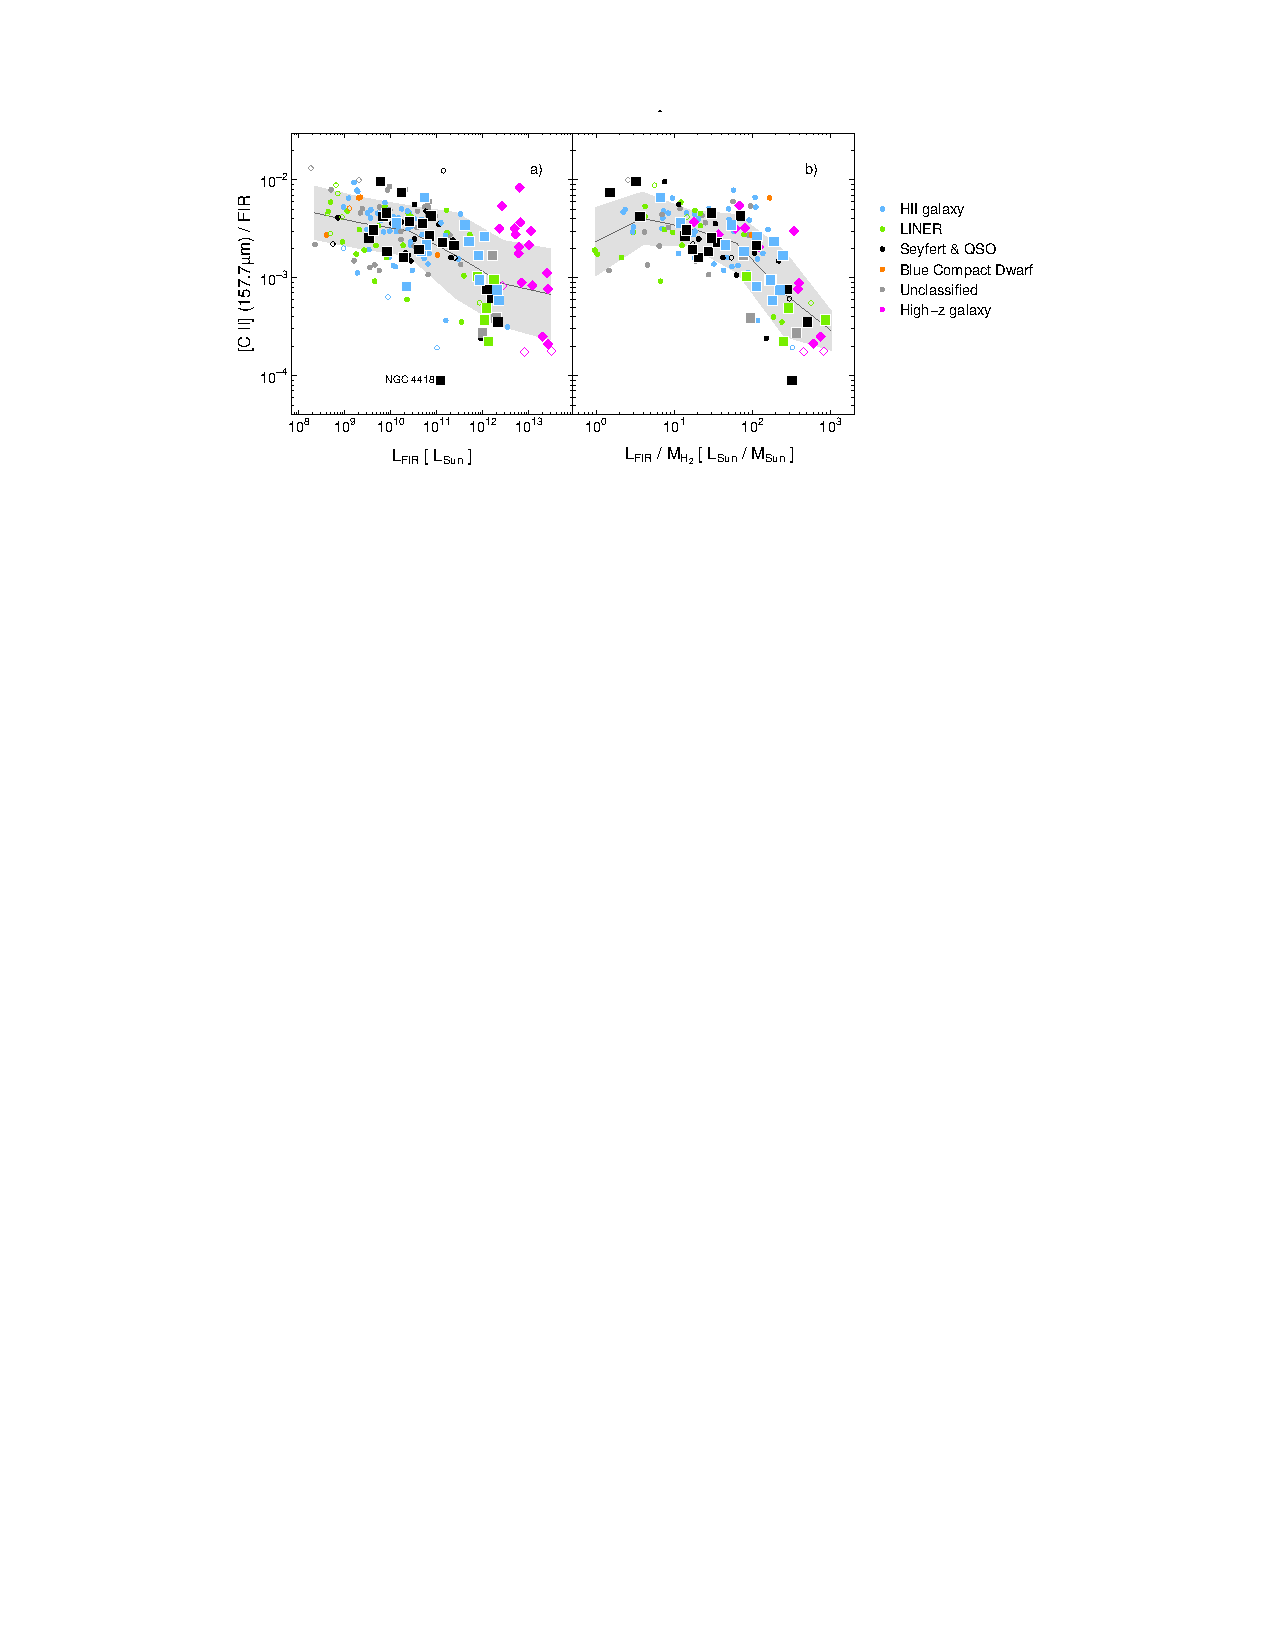
\includegraphics[width=4.5in]{gracia-carpio11_fig1.pdf}
      \end{center}     
    \end{minipage} &
    \begin{minipage}{2in}
      \begin{center}
	\caption{\small {\it Left:} The correlation between \cii\ luminosity
and FIR luminosity for individual galaxies and the $L_{FIR}/M_{H_2}$
relation (as compiled in \citet{gracia-carpio11}.)}
% {\it Right:}
% Expected numbers of detections of galaxies above $5\sigma$ (long
% dashed) and $1\sigma$ (dotted) across the range of redshifts probed by
% \name, based on the number counts of \citet{bethermin12} and the
% observed $L_{[CII]}-L_{FIR}$ relation.}
      \end{center}
    \end{minipage}
  \end{tabular}
 
\label{fig:LCII-LFIR}
\end{figure}

% \begin{figure}[h]
%   \begin{tabular}{ll}
%     \begin{minipage}{3.25in}
%       \begin{center}
% 	\includegraphics[width=3.25in]{sim_blast500.pdf}
%       \end{center}
%     \end{minipage} &
%     \begin{minipage}{3.25in}
%       \begin{center}
% 	\includegraphics[width=3.25in]{sim_channel_map.pdf}
%       \end{center}
%     \end{minipage} \\
%     \begin{minipage}{3.25in}
%       \begin{center}
% 	\includegraphics[width=3.25in]{sim_cii_dist.pdf}
%       \end{center}
%     \end{minipage} &
%     \begin{minipage}{3.25in}
%       \begin{center}
% 	\includegraphics[width=3.25in]{sim_spectrum.pdf}
%       \end{center}
%     \end{minipage}
%   \end{tabular}
%     \caption {\small {\it Upper left:} Continuum image from a
%     simulated \name\ data cube showing the co-addition of spectral
%     channels.  {\it Upper right:} A single spectral channel, showing a
%     detected source.  {\it Bottom left:} Slices of the data cube are
%     amenable to $P(D)$ analysis, as in \Citet{patanchon09} or
%     \citet{glenn10}, to extract the luminosity function of \cii, or
%     the number counts of the continuum.  {\it Bottom right}: A
%     spectrum of the individually detected galaxy. The continuum has
%     been subtracted at each spatial pixel using a 3rd order polynomial.}
% \label{fig:IMapping}
% \end{figure}

\begin{figure}[h]
  \begin{tabular}{ll}
    \begin{minipage}{3.25in}
      \begin{center}
	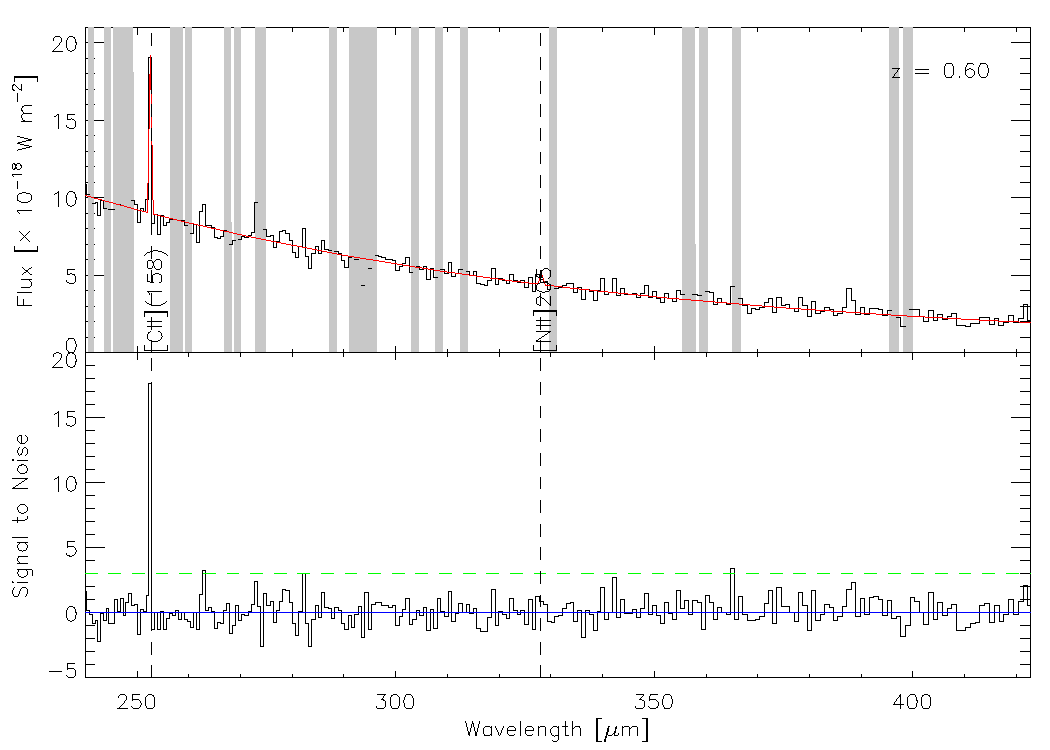
\includegraphics[width=3.25in]{simgal_z060.pdf}
      \end{center}
    \end{minipage} &
    \begin{minipage}{3.25in}
      \begin{center}
	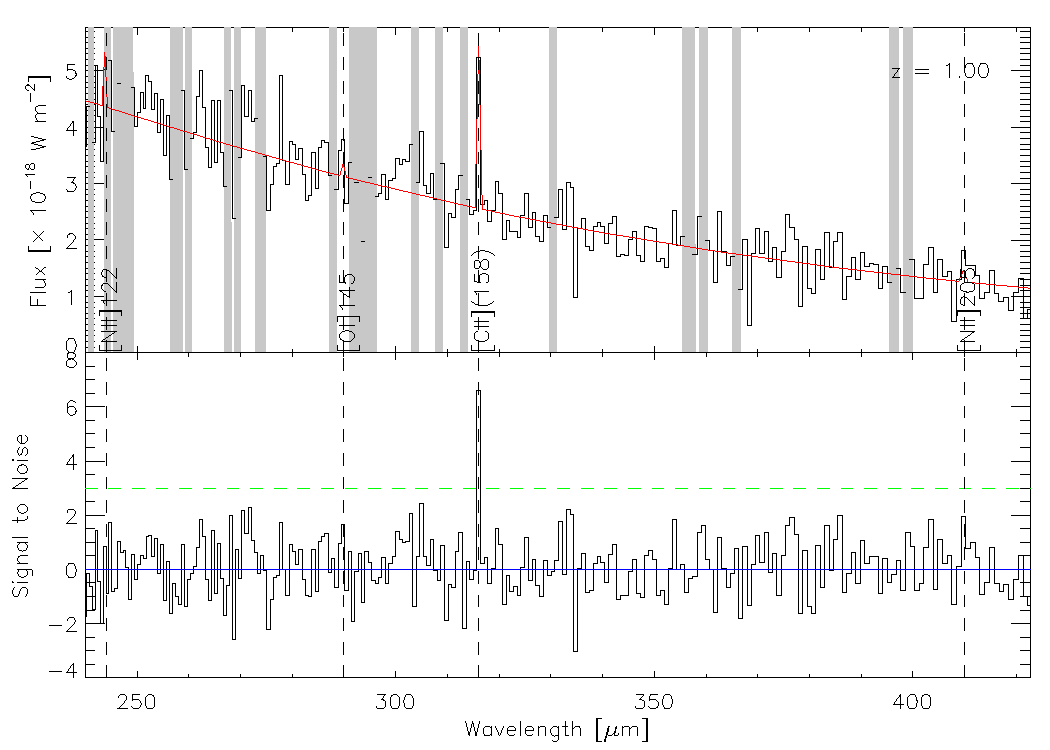
\includegraphics[width=3.25in]{simgal_z100.pdf}
      \end{center}
    \end{minipage} \\
    \begin{minipage}{3.25in}
      \begin{center}
	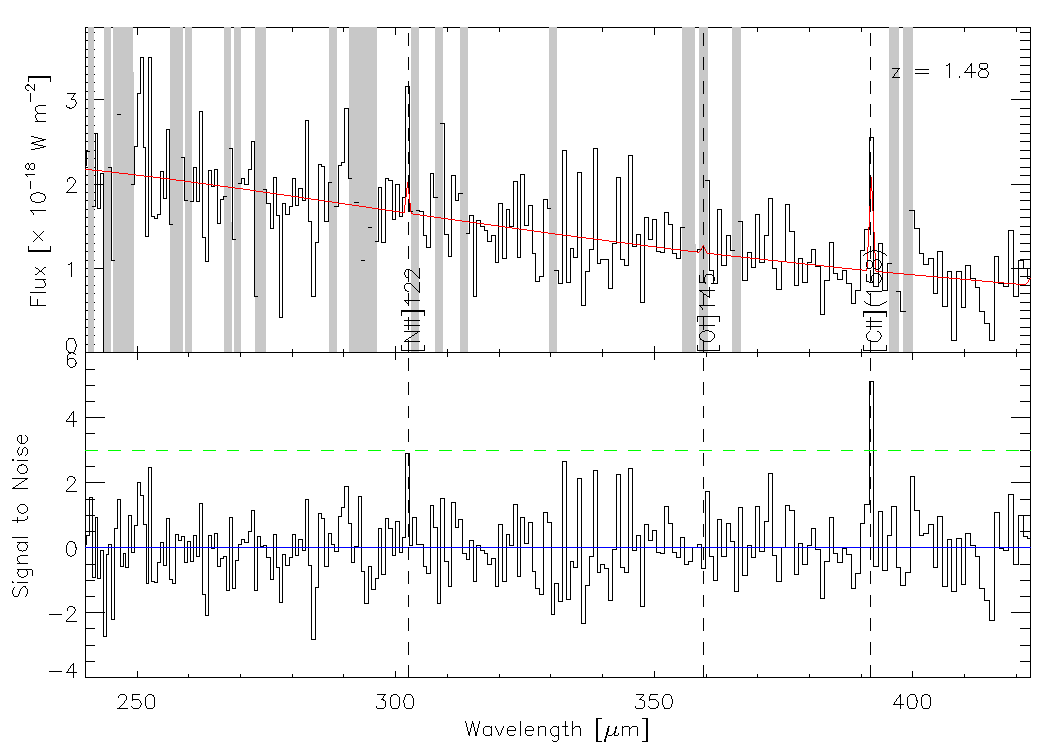
\includegraphics[width=3.25in]{simgal_z148.pdf}
      \end{center}
    \end{minipage} &
    \begin{minipage}{3.25in}
      \begin{center}
	\caption {\small Simulated spectra of galaxies with $L_{FIR}=4\times10^{12}~\Lsun$ at various redshifts for which \cii\ is accessible to \name.  The observations assumed only 10 minutes of integration time.  Note that in addition to the \cii\ line, the continuum is strongly detectect ($T_{dust}=35$~K is assumed), allowing for unambiguous checks on the pointing and calibration.  Channels with $2\times$ higher noise than the median are shown in gray (approximately 11\% of the total), but the lower panel of each figure shows the signal-to-noise accounting for this increased variance, indicating that these channels, while less sensitive, do not create false positives.}
	\label{fig:SimGalaxies}
	\end{center}
    \end{minipage}
  \end{tabular}
    
\label{fig:IMapping}
\end{figure}

\begin{figure}[h]
  \begin{tabular}{ll}
    \begin{minipage}{3.25in}
      \begin{center}
	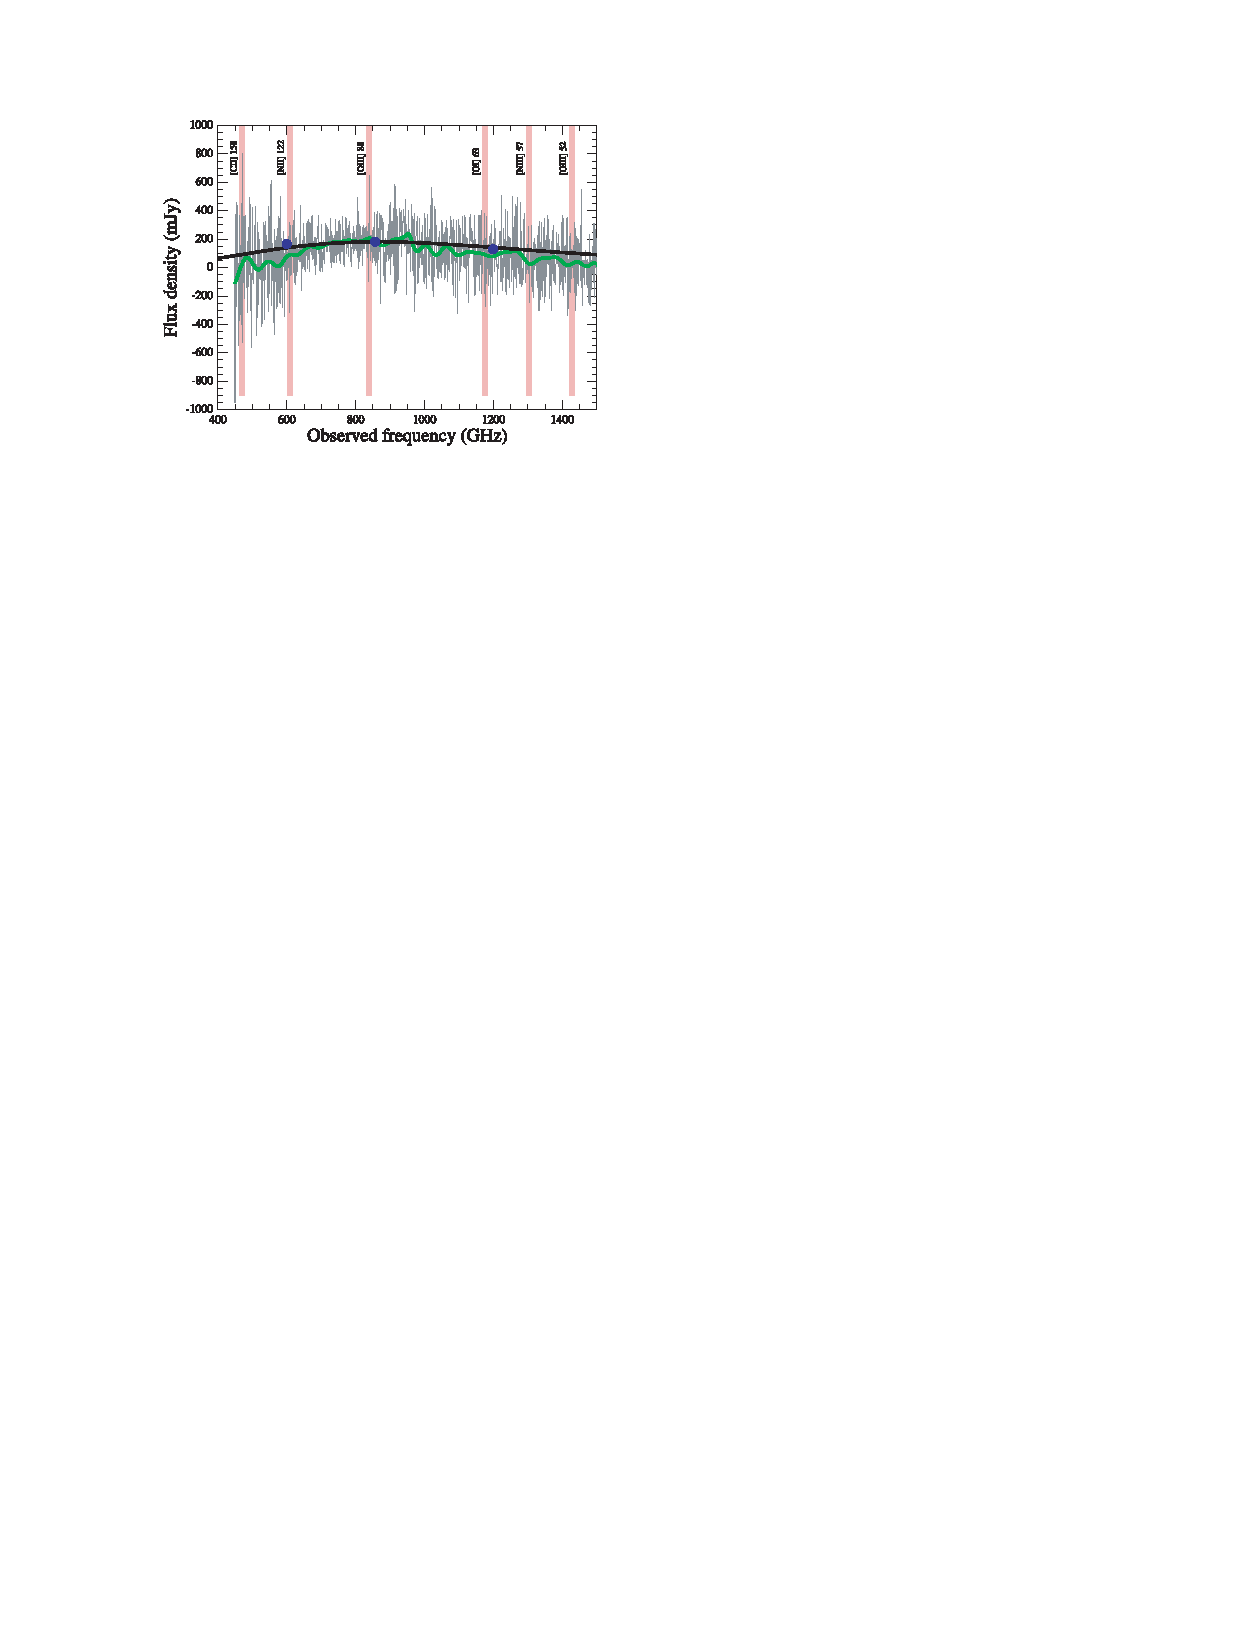
\includegraphics[width=3.25in]{valtchanov11_sdp81_spire_fts_spectrum.pdf}
      \end{center}
    \end{minipage} &
    \begin{minipage}{3.25in}
      \begin{center}
	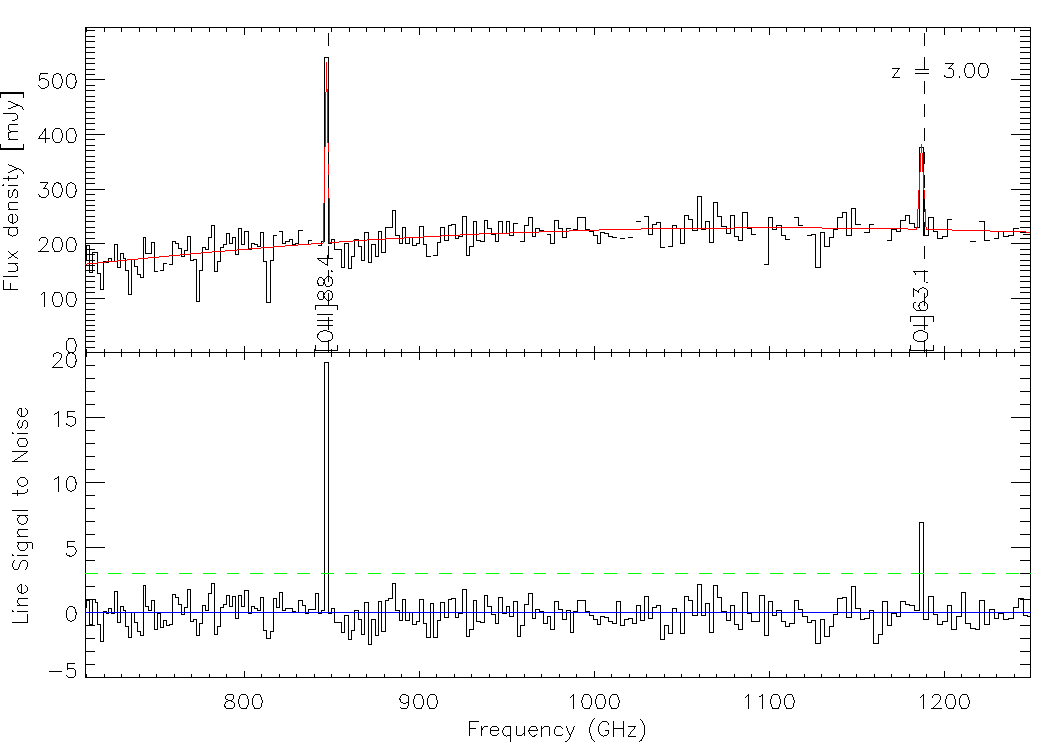
\includegraphics[width=3.25in]{simgal_z300.pdf}
      \end{center}
    \end{minipage} 
  \end{tabular}
    \caption {\small {\it Left:} The \herschel-SPIRE FTS spectrum of SDP.81 from \citet{valtchanov11}, representing nearly 4 hours of integration time.  This galaxy was, at the time of publication, the faintest \cii\ line yet detected by \herschel.  {\it Right:} A similar galaxy observed for 10 minutes with \name.  Though \cii\ has redshifted out of the \name\ band, note the clear detection of \oiii (52 \mum) as well as \oiii (88 \mum).}
\end{figure}

\subsubsection{Power Spectrum of \cii (Science Goal \ref{goal:PowerSpectrum})}

Our overarching goal is to connect the process of star formation in
individual galaxies via their average properties to the properties of
large scale structure (LSS).  To do this requires mapping a large
cosmic volume, and in addition, traditionally requires large
spectroscopic redshift surveys coupled with careful attention to
obtaining photometry for photometric redshifts.  However, in the
far-IR, the process of obtaining redshifts is difficult and slow.
However, the traditional route can be circumvented by {\it intensity
mapping}: making a large data cube in which the third dimension
measured a line, thus providing redshift information.
%\footnote{We note
%that intensity mapping is not a replacement for traditional galaxy
%surveys or detailed studies of individual galaxies, but is rather a
%highly complementary addition to the information gained from them, and
%can profitably be combined with them.  In particular, it provides a
%way of measuring galaxy properties at the clustering scale with small
%error bars and also allows the measurement of the average properties
%of low surface brightness galaxies.}.  
In general, individual galaxies
are not detected, and the information is extracted from the data via a
power spectrum or cross-spectrum.

The most developed case for intensity mapping is that of the 21 cm
experiments attempting to detect the epoch of reionization.\footnote{PI
Aguirre is currently co-PI of NSF AST 1125558 ``Collaborative
Research: Precision Array for Probing the Epoch of Reionization
(PAPER)''.  PAPER is a dedicated attempt to detect the highly
redshifted 21 cm emission from the epoch of reionization.}  At $z \sim
1$, intensity mapping using \hi\ has been proposed for measuring
baryon acoustic oscillations \citep[BAO][]{chang08} and the concept
experimentally demonstrated by the detection of the cross-spectrum of
\hi\ emission with the DEEP2 galaxy survey \citep{chang10}.  Several
theoretical studies have recently been published demonstrating the
feasibility of doing intensity mapping during the epoch of
reionization using CO, \cii\ and other transitions in large-beam
surveys
\citep{carilli11,lidz11,gong11co,gong11cii,visbal11,visbal10}.
% \footnote{We
% also note an experiment described in \citet{zemcov11} similar in
% spirit to intensity mapping, which is attempting to detect the
% signature of the first stars from spectrally-discriminated
% fluctuations in the near-infrared background.}.

With this in mind, we begin by considering the line emission from some
particular species $i$ present in the ISM of galaxies.  (We assume any
continuum contribution has been removed; this is actually
straightforwardly achieved, following schemes which use the spectral
smoothness of the continuum to subtract it.  See, for example,
\citet{bowman09}.)  We have an instrument which acts as an integral
field spectrometer, mapping an intensity data cube
$S(\alpha,\delta,\nu)$, where $(\alpha,\delta)$ are the celestial
coordinates of the line-of-sight along which the spectral frequency
dimension $\nu$ is measured.  Since we are working with line emission,
the observed frequency determines the cosmological redshift and thus
$\nu$ may be transformed into line-of-sight distance, and for each
distance, a transverse dimension may also be obtained.  Thus
$S(\alpha,\delta,\nu) \Leftrightarrow S(\vect{x})$, where $\vect{x}$
denotes comoving spatial coordinates.  The logic of this argument is
laid out for the 21 cm \hi\ fluctuations in, for example,
\citet{morales05}.  We assume that the extent of $\vect{x}$ in the
cube is such that significant cosmological evolution does not occur
over the measured region.

Since the galaxies whose line emission we are measuring trace the
underlying dark matter potential (with some bias), the intensity field
of line emission fluctuations can be written as
\begin{equation}
\Delta S_i(\vect{x}) = \bar{S}_i \bar{b} \delta(\vect{x})
\end{equation}
where $\bar{S}_i$ is average emission line signal, $\bar{b}$ is
luminosity weighted average galaxy bias, and $\delta(\vect{x})$ is the
cosmological overdensity at $\vect{x}$.  In general, since for any
realistic instrument the signal-to-noise at any point $\vect{x}$ will
be low, we will be concerned with the statistical measures on $S$.  In
particular, the power spectrum
% \footnote{Historically, the presence of
% a non-zero-mean instrument noise term (and its corresponding bias) was
% a cause for considerable concern in using the auto-spectrum.  However,
% with multiple measurements of $\Delta S_i(\vect{x})$, it is possible to
% construct auto-spectrum estimators which are unbiased, and thus this
% concern can be removed by proper instrument and observing design
% \citep[e.g., ][]{polenta05,tristram06}.} 
of such a signal is
\begin{equation}
P_i(k) = \bar{S}_i^2 (\bar{b}^2 P(k) + P_s)
\end{equation}
where $P(k)$ is the matter power spectrum, and we have made the usual
assumption of isotropy in the fluctuations.  $P_s$ is a shot (or
Poisson) noise term due to the fluctuations of uncorrelated, discrete
galaxies, from which we have factored the average line brightness.
Note that at the angular scales measured by \name, the clustering
term dominates over the shot noise.  Figure \ref{fig:PowerSpectrum}
shows that a future LDB experiment similar to \name\ with 200 hours of integration would be able to measure the power spectrum of \cii\ emitters with high
signal-to-noise over a range of redshifts and angular scales,
accurately measuring the clustering signal.  With this proposal, we have the sensitivity to detect the highest-$k$ shot noise and set the scale of the \cii\ fluctuations.

% A concern in using the power spectrum of a given line, as has been
% pointed out by \citet{visbal11} and others, is that it may be
% contaminated by foreground line emission from ``interloper lines''
% (lines which share the same observed frequency but not the same
% redshift).  We show the effect of interloper lines for \name\ in
% Figure \ref{fig:AccessibleLines}.  In general, these are expected to
% be fainter than \cii, and at higher redshift.  One way, however, of
% rejecting such interlopers is to use the cross power spectrum of two
% distinct lines
% \begin{equation}
% P_{i,j}(k) = \bar{S_i} \bar{S_j} (\bar{b}^2 P(k) + P_s)
% \end{equation} 
% since interloper lines not at the same redshift will generally be
% uncorrelated in the cross spectrum.  For \name, as shown in Figure
% \ref{fig:AccessibleLines}, the \nii(122), \nii(205), and \oi(145)
% lines are all available for cross-correlation over some portion of the
% redshift range sampled by \cii.  We show that we can detect the
% \cii-\nii\ cross-correlation at $z\sim1$ in Figure
% \ref{fig:NIICrossCorr}.  We will use such a cross-correlation to aid
% in rejecting systematic contamination of the \cii\ power spectra.
% 
% In addition to its role in producing cross-spectra, \nii\ is
% astrophysically interesting in its own right.  It is useful for
% measuring the (unextincted) star-formation rate, and is the basis for
% one of the best measurements in the Galaxy \citep{bennett94}.  The
% 205\mum\ \nii\ line also provides a vital key to the interpretation of
% the \cii\ line.  Because its ionization potential is only 11.3 eV,
% \cii\ may exist in regions of both neutral and ionized hydrogen.
% \nii\ and \cii\ have nearly identical critical densities and second
% ionization potentials (29.6 and 24.4 eV, respectively), so the \nii /
% \cii\ ratio is sensitive only to the relative abundances of the two.
% However, since nitrogen has an ionization potential of 14.5 eV, it is
% present only in ionized hydrogen gas, and thus the ratio
% \cii/\nii(205) probes the fraction of \cii\ present in ionized regions
% \Citep{oberst06}.  This information provides an essential insight into
% the physical origins of the \cii\ emission.
% 
% Flux ratios of emission lines offer a powerful means of extracting
% astrophysics from line emission by constructing quantities in which
% some unknown factor - a physical parameter of the gas - cancels, thus
% allowing the isolation of a particular effect due to the unknown
% physical parameter under investigation
% \citep{osterbrock89,spinoglio92}.  For ionized tracers, different
% lines from the same ion trace {\it density}, as the electron
% temperature is much larger than the relevant energy levels, and the
% abundance drops out. A good example relevant to \name\ is
% \nii(122)/\nii(205). For neutral gas tracers, the gas temperature is
% now no longer necessarily larger than the relevant energy levels, so
% both density and temperature are important. A good example is
% \cii(158)/\oi(145).  The \oi(145) line has a higher critical density
% and upper energy level than \cii, and so the \oi/\cii\ ratio traces
% the combined effects of high densities and temperatures in PDRs
% \citep{malhotra01}.  The cross-spectra of three lines allows the
% construction of two line ratios which are again resistant to
% foreground contamination:
% \begin{equation}
% \frac{P_{l,n}(k)}{P_{m,n}(k)} = \frac{\bar{S}_l}{\bar{S}_m} 
% \equiv R_{l,m}
% \end{equation}
% Using all lines available to us, we will construct these line ratios,
% making detections or constraining their values over a range of
% redshifts.

\begin{figure}[h]
  \begin{tabular}{ll}%{p{3.0in}@{\hspace{0.6in}}p{3.0in}}
    \begin{minipage}{3.25in}% \vspace{-.2in} 
      \begin{center} %\hspace{+0.79in}
	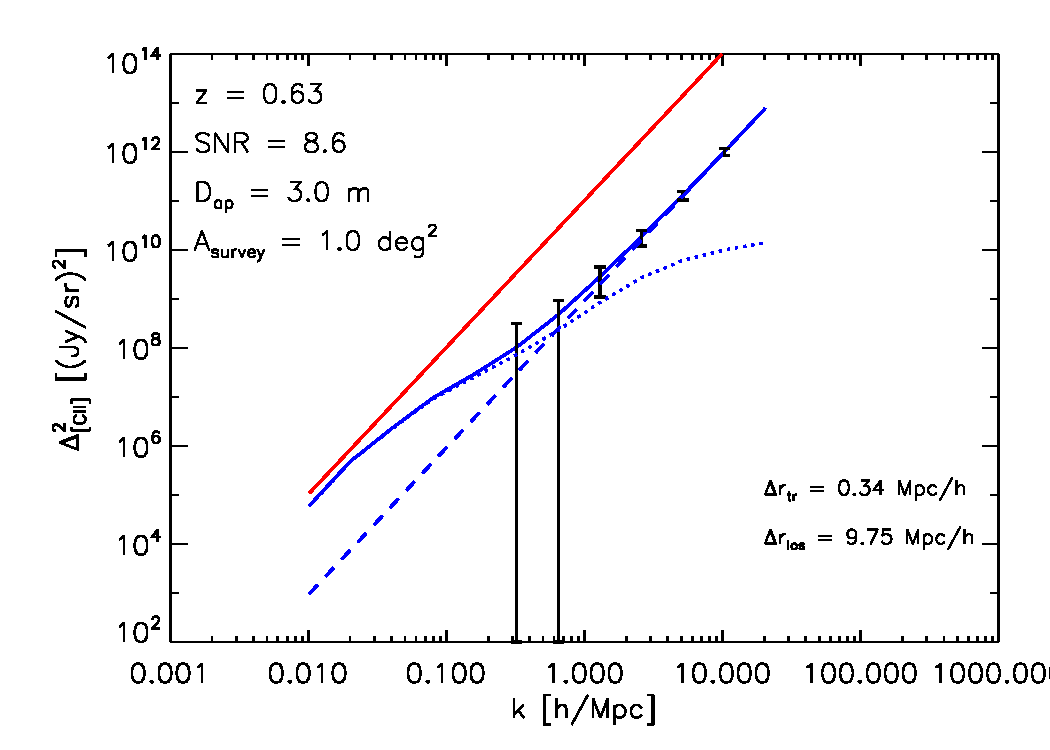
\includegraphics[width=3.25in]{pcii_z63.pdf}
	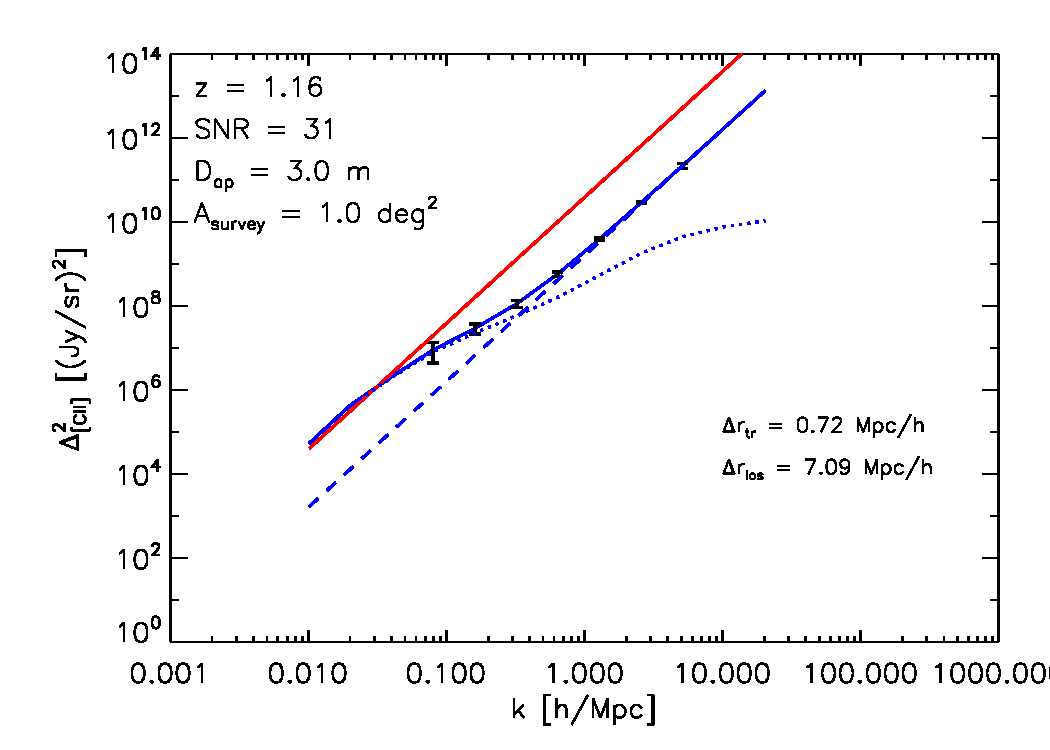
\includegraphics[width=3.25in]{pcii_z116.pdf}
      \end{center}
    \end{minipage} &
    
    \begin{minipage}{3.25in}% \vspace{-.6in}
      \begin{center}% \hspace{+0.79in}
	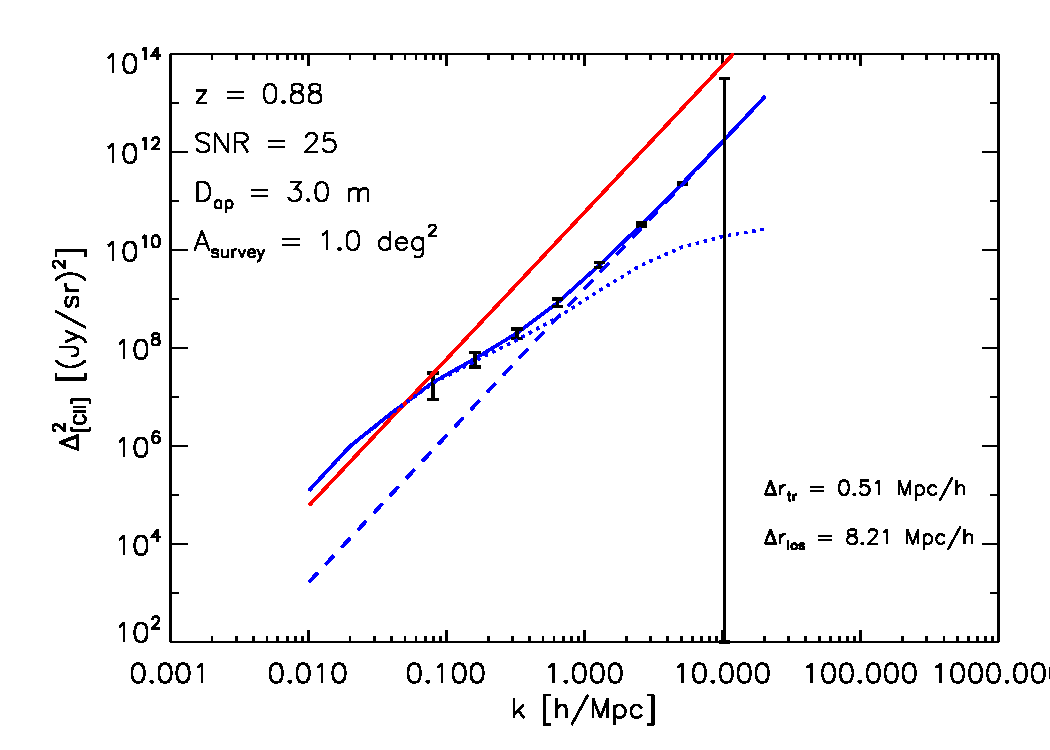
\includegraphics[width=3.25in]{pcii_z88.pdf}
	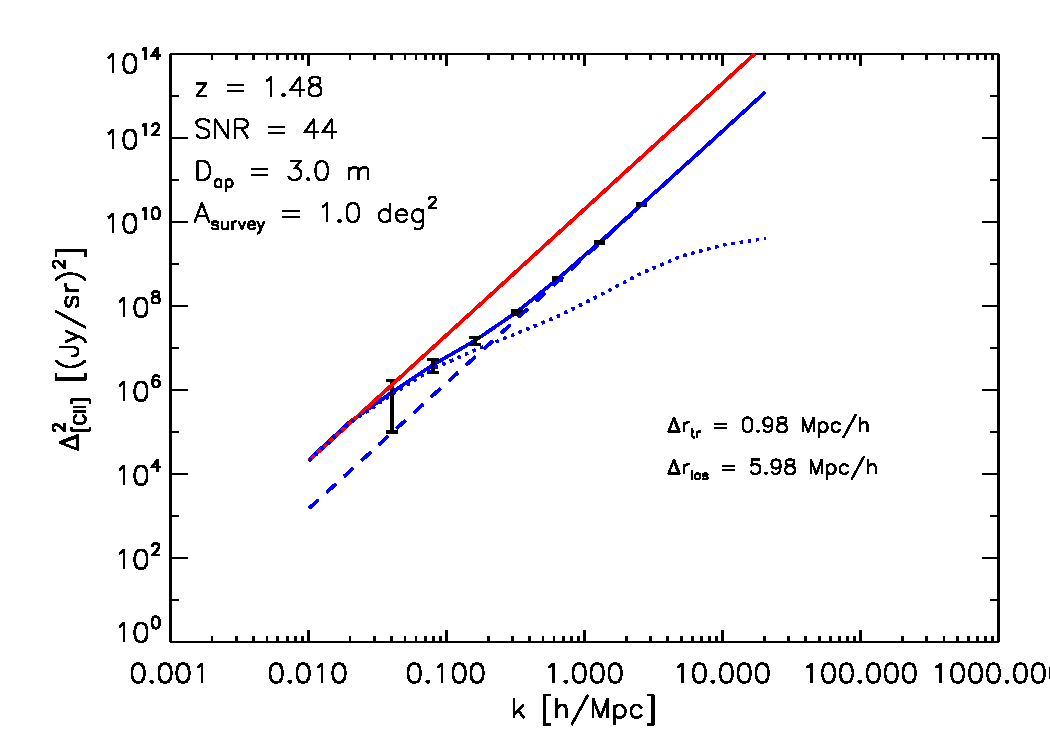
\includegraphics[width=3.25in]{pcii_z148.pdf}
      \end{center}
    \end{minipage}
  \end{tabular}
    \caption {\small Predicted power spectra for the \cii\ line at
    four redshifts.  Dashed lines show the one- and two-halo
    clustering terms, and the dotted line shows ``shot noise'' or
    Poisson term from unclustered galaxies.  Note that the clustering
    raises the amplitude of the power spectrum many orders of
    magnitude above the shot noise expectation.  The vertical black
    dash-dotted lines indicate the range of sales probed by \name,
    i.e., those between $[(2 \pi)^3/V_s]^{1/3}$ and
    $[(2\pi)^3/V_{pix}]^{1/3}$, where $V_s$ and $V_{pix}$ are total
    survey volume and pixel volume respectively.}
\label{fig:PowerSpectrum}
\end{figure}

% \begin{figure}[h]
%   \begin{tabular}{ll}
%     \begin{minipage}{3.25in}
%       \begin{center}
% 	\includegraphics[width=3.25in]{P_CIINII_z1.pdf}
%       \end{center}     
%     \end{minipage} &
%     \begin{minipage}{3.25in}
%       \begin{center}
% 	\caption {\small At $z=1$ both \nii(205~\mum) and
% 	\nii(122~\mum) are available for cross-correlation with \cii\
% 	in the \name\ bands.  Here we show the amplitude of the
% 	cross correlation assuming $b_{CII}=b_{NII}=2.5$, and
% 	$I_{NII}=(0.13+0.05)I_{CII}$, i.e., using a fiducial ratio for
% 	\cii\ to \nii\ emission.  The \nii\ cross-correlation is
% 	particularly important, as it helps to calibrate the relative
% 	fraction of \cii\ emission coming from \hii\ regions versus
% 	those dominated by \hi.}
% 	\label{fig:NIICrossCorr}
%       \end{center}
%     \end{minipage}
%   \end{tabular}
% 
% \end{figure}
% 
% \begin{figure}[h]
%   \begin{tabular}{ll}
%     \begin{minipage}{3in}
%       \begin{center}
% 	\includegraphics[width=3in]{icaris_accessible_lines.pdf}
%       \end{center}     
%     \end{minipage} &
%     \begin{minipage}{3.5in}
%       \begin{center}
% 	\includegraphics[width=3.5in]{line_ratios.pdf}
%       \end{center}
%     \end{minipage}
%   \end{tabular}
% 	\caption {\small {\it Left:} Lines accessible in the \name\
% 	band, as well as potential low- and high-redshift interlopers.
% 	Lines available for cross-correlation with \cii\ at the same
% 	redshift lie between the horizontal black lines.  Interlopers
% 	appearing at the same observed wavelength but different
% 	redshift may be read off along vertical lines.  Interloper
% 	lines at higher redshift than we will map with \cii\ are all
% 	intrinsically fainter than \cii, in addition to their
% 	cosmological dimming.  At lower redshifts, the dominant
% 	contaminants will be high-$J$ lines of CO at redshifts $z<0.5$
% 	Galaxies exhibiting such lines will tend to (U)LIRGs
% 	detectable in the IRAS surveys.  We can also use \herschel\
% 	surveys to identify low-$z$ interlopers. {\it Right:} The
% 	relative strengths of far-IR lines, as observed in M82. \cii\
% 	dominates all lines except \nii(205), with which it will be
% 	cross-correlated.}
% 	\label{fig:AccessibleLines}
% \end{figure}

